% Participation
\newcommand{\totalkeys}{78}
\newcommand{\usableparticipants}{42}
\newcommand{\scrappedparticipants}{13}
\newcommand{\expcount}{21}
\newcommand{\ctlcount}{21}

% Experience
\newcommand{\inexpdebug}{19}
\newcommand{\expdebug}{23}
\newcommand{\inexpvuln}{30}
\newcommand{\expvuln}{12}


% Correctness
\newcommand{\expmediancorrect}{5}
    \newcommand{\inexperiencedexpmediancorrect}{1}
    \newcommand{\experiencedexpmediancorrect}{4}
\newcommand{\expfollowcorrect}{14}
    \newcommand{\inexperiencedexpfollowcorrect}{7}
    \newcommand{\experiencedexpfollowcorrect}{7}
\newcommand{\expnotescorrect}{14}
    \newcommand{\inexperiencedexpnotescorrect}{6}
    \newcommand{\experiencedexpnotescorrect}{8}
\newcommand{\ctlmediancorrect}{7}
\newcommand{\ctlfollowcorrect}{7}
\newcommand{\ctlnotescorrect}{11}


\chapter{RESULTS}
\section{Participants}
Participants were sourced primarily from a variety of cybersecurity-oriented Discord servers, as members in these groups would have a higher chance of having the requisite skills to complete the experiment. Initially, members were primarily recruited from Discord servers created for various undergraduate and graduate cybersecurity courses offered at Arizona State University. Once this pool was depleted, recruitment messages were sent to various reverse-engineering oriented Discord servers with members from around the globe. These servers provided a sufficient pool of enthusiastic participants.

A total of \totalkeys{} session keys were sent out to individuals who had expressed interest in participation, whether through email or by responding to the Discord recruitment messages. To incentivize participation, participants were awarded \$50 for completion of the entire study. As a result, there was a turnout of \usableparticipants{} participants who fully completed the study. An additional \scrappedparticipants{} participants had their data thrown out, as they either partially completed the experiment or were unable to participate due to RDP latency or other technical difficulties.

Of the participants who fully completed the experiment, \inexpdebug{} had less than 2 years of experience in software debugging and \expdebug{} had 2+ years. As for vulnerability analysis experience, \inexpvuln{} had less than 2 years of experience and \expvuln{} had 2+ years. In order to differentiate between these experience groupings, participants with less than 2 years of experience in a subject will be referred to as being 'inexperienced' while those with 2+ years will be referred to as 'experienced'.

\section{Challenge Correctness}
\begin{table}
    \begin{center}
        \caption{Aggregated Challenge Results}
        \label{table:challscore}
        \begin{tabular}{@{}lcccc@{}}
        \toprule
        \textbf{Group} & \textbf{Pass} & \textbf{Fail} & \textbf{P-value} \\
        \midrule
        \textbf{Control} \\
            \hspace{3mm}Median & \ctlmediancorrect{} & \fpeval{\ctlcount{} - \ctlmediancorrect{}} & 0.753 \\
            \hspace{3mm}Follow & \ctlfollowcorrect{} & \fpeval{\ctlcount{} - \ctlfollowcorrect{}} & 0.015 \\
            \hspace{3mm}Notes & \ctlnotescorrect{} & \fpeval{\ctlcount{} - \ctlnotescorrect{}} & 0.173 \\
        \midrule
        \textbf{Experiment} \\
            \hspace{3mm}Median & \expmediancorrect{} & \fpeval{\expcount{} - \expmediancorrect{}} \\
            \hspace{3mm}Follow & \expfollowcorrect{} & \fpeval{\expcount{} - \expfollowcorrect{}} \\
            \hspace{3mm}Notes & \expnotescorrect{} & \fpeval{\expcount{} - \expnotescorrect{}} \\
        \end{tabular}
    \end{center}
\end{table}

Each participant's challenge questionnaire was scored on a binary scoring system, with 1 point being awarded for the correct answer and 0 for the incorrect answer. As the same grading criteria was applied to control and experimental submissions, the opportunity for biased grading was eliminated. Table \ref{table:challscore} summarizes the results of the challenge-solving portion of the experiment. The experimental group saw better performance when solving the follow and notes challenges. In fact, a 100\% improvement was seen in solve percentage between the control and experiment group in the follow challenge. This was determined to be a statistically significant difference, showing that data dependency view is a contributor to improved performance in regard to this challenge. However, there were not enough samples or variance to determine statistical significance for the notes and median challenges. Due to the marginal differences between notes and median solves, the P-value of correctness between the groups is 0.076. If the standard 95\% confidence interval is used, this is just barely outside the range required to reject the null hypothesis. Within this specific participant pool, the control group was more likely to solve the median challenge. This unexpected result could be due to the wording of the median questionnaire, as it proved confusing to participants. Thus, this marginal difference could be explained by a poorly designed challenge with poor questions. The fact that follow, a challenge based on making sense of a complicated chain of data dependencies, saw a significantly higher solve-rate amongst the experiment group while notes and median saw marginal improvements and degressions speaks to the reality that data dependency graph analysis is a specialized tool. While it is provably effective in the specific domain of resolving data dependencies, improvement gains are less dramatic in other realms of binary analysis. Due to both the ten minute attempt suggestion given to challenges and the need to keep challenges feasibly solvable within that time frame, it is difficult to capture an element of data dependency in every challenge.

Unsurprisingly, users with more experience in software debugging performed better on the software debugging challenges: median and notes. Of the \expmediancorrect{} solves for median in the experimental group, \experiencedexpmediancorrect{} came from experienced software debuggers. As for notes, \experiencedexpnotescorrect{} of the \expnotescorrect{} solves came from participants with a strong debugging background. This shows that data dependency graph analysis is an effective software debugging tool that can be judiciously applied by the experienced software debugger. To further support this notion, follow, a challenge without elements of software debugging, saw the same performance among inexperienced and experienced software debuggers. Similarly, experience with vulnerability analysis had no discernible impact on challenge correctness. This shows that data dependency graph should not be advertised as a vulnerability analysis tool. 

\section{Completion Time}

\definecolor{bblue}{HTML}{4F81BD}
\definecolor{rred}{HTML}{C0504D}

\begin{figure}[!htb]
    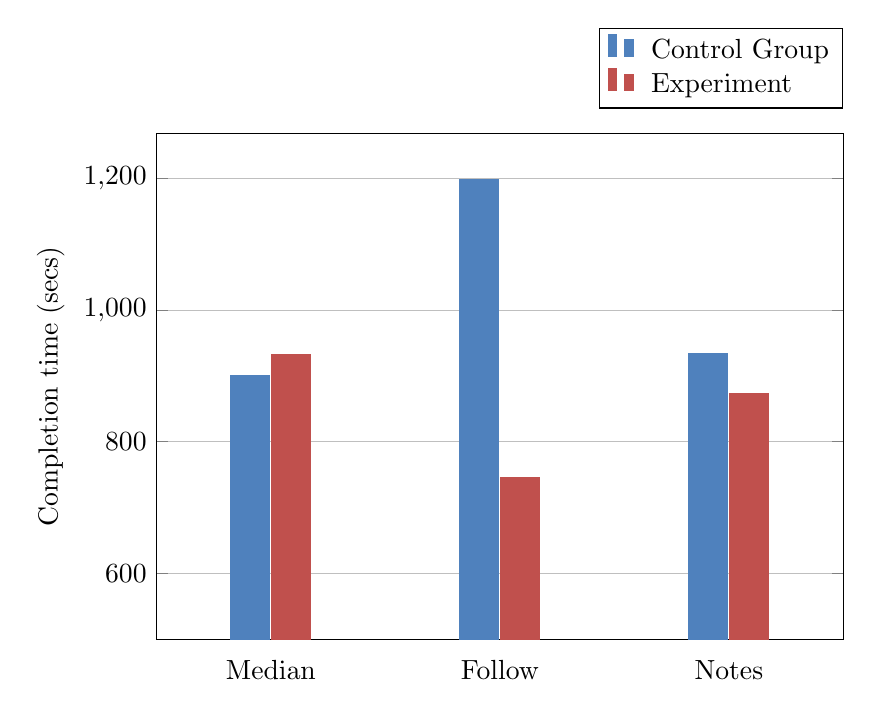
\begin{tikzpicture}
        \begin{axis}[
            width  = 0.85*\textwidth,
            height = 8cm,
            major x tick style = transparent,
            ybar=2*\pgflinewidth,
            bar width=14pt,
            ymajorgrids = true,
            ylabel = {Completion time (secs)},
            symbolic x coords={Median,Follow,Notes},
            xtick = data,
            scaled y ticks = false,
            enlarge x limits=0.25,
            ymin=500,
            legend cell align=left,
            legend style={
                    at={(1,1.05)},
                    anchor=south east,
                    column sep=1ex
            }
        ]
            \addplot[style={bblue,fill=bblue,mark=none}]
                coordinates {(Median, 900) (Follow, 1198) (Notes, 934)};
    
            \addplot[style={rred,fill=rred,mark=none}]
                 coordinates {(Median, 932) (Follow, 745) (Notes, 873)};
    
            \legend{Control Group, Experiment}
        \end{axis}
    \end{tikzpicture}
    \caption{Completion time results}
    \label{fig:time}
\end{figure}
The average completion time of each challenge was computed for the experiment and control groups. Only participants who were able to get the correct answer were incorporated into these calculations, as the speed it takes a participant to derive an incorrect answer is irrelevant. As many participants were unable to get the correct answer, fewer data points were able to be considered. The only conclusive statistical result was, again, in the follow challenge. When using a 95\% confidence interval, the null hypothesis stating that data dependency view resulted in faster solves on average, could not be rejected with a P-value of P=0.132. Although, the results within the participant pool show a trend for solving challenges faster using data dependency graph. The only challenge that saw poorer performance with data dependency graph was median, which could be attributed to the extremely small sample size of participants who were able to solve the challenge. Despite the experiment group solving challenges 171 seconds faster on average, no statistical significance can be determined with the data. This could possibly be attributed to the user's being provided a ten minute timer for challenge-solving, which eliminates the majority of the possible variance.

Experienced software debuggers in the experimental group saw over a 200\% speedup in completion time for solving median, cementing the importance of software debugging knowledge in solving this challenge. No correlation between software debugging expertise and completion time was exhibited by the other two challenges. As for experience with vulnerability analysis, those with experience saw a 185\% speedup in completion time for solving notes. This may be attributed to the fact that the challenge was modeled after a common CTF challenge format, which was commented on in many participant's feedback for that challenge. 

\section{User Perception}
\begin{figure}[!ht]
    \centering
    \begin{subfigure}[a]{0.75\textwidth}
        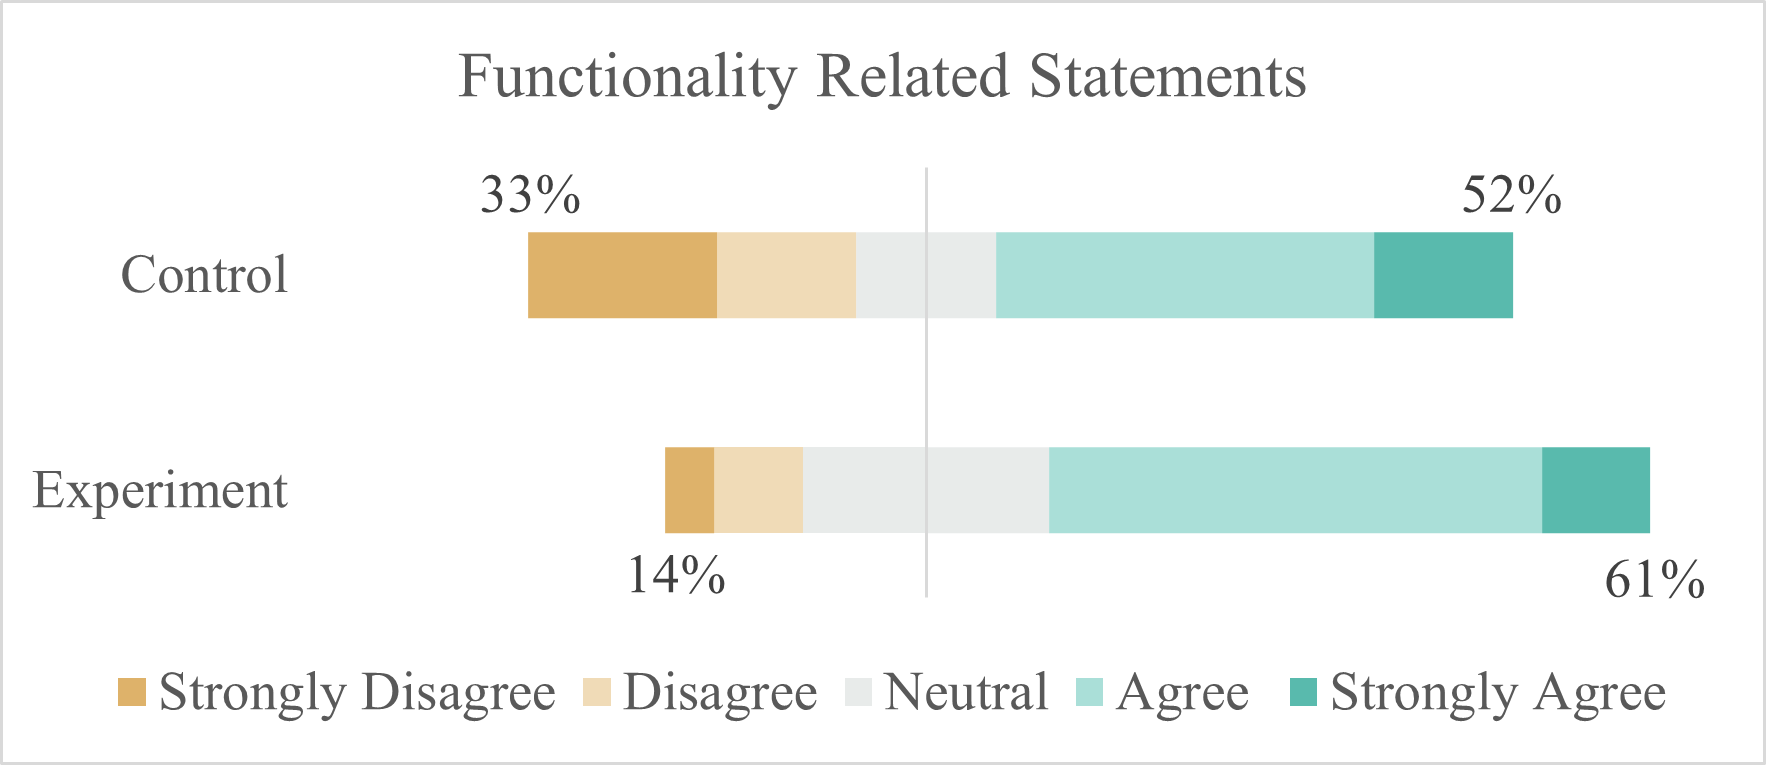
\includegraphics[width=1\linewidth]{functionalitygraph.png}
        \caption{}
        \label{fig:functionality}
    \end{subfigure}
    
    \begin{subfigure}[b]{0.75\textwidth}
        \centering
        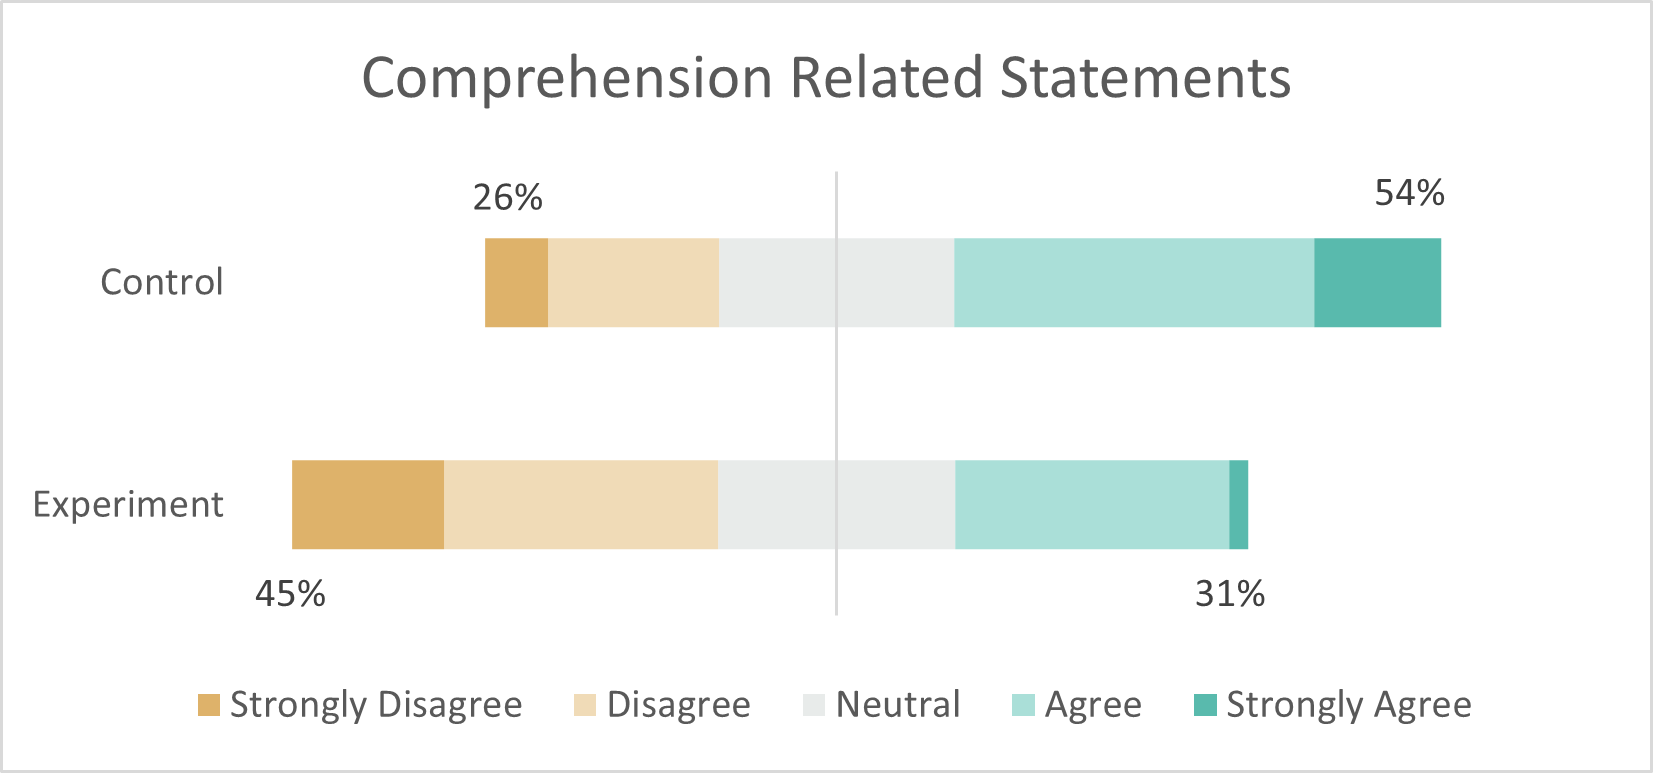
\includegraphics[width=1\linewidth]{comprehensiongraph.png}
        \caption{}
        \label{fig:comprehension}
    \end{subfigure}
    \caption{Aggregated participant agreement with the statements related to (a) functionality and (b) comprehension}
\end{figure}
In addition to the quantitative data that was gathered, participants were also asked to provide their general feedback at the end of the experiment. The full list of survey questions can be seen in Appendix B. Figures \ref{fig:functionality} and \ref{fig:comprehension} provide a summary of the user's perception. Questions were aggregated into two groups: comprehension related (questions 7\&8 for control and 7\&13-14 for experiment) and functionality related (9 for control and 8-12 for experiment). User feedback communicates that the experimental group generally viewed the functionality of the view favorably, but viewed its comprehensibility negatively. This communicates that the analysis itself is a useful addition to the suite of \code{angr} analyses, but the user interface requires rework to be more in line with user expectations. 

In addition to asking the experimental group for feedback on the data dependency view, users in the control group were asked two questions about a "hypothetical" data dependency view in the post-participation survey. The control group was given an example screenshot of a simple data dependency graph, depicted in Figure \ref{fig:motivddg}, and asked if they thought that the hypothetical view would be helpful. They were then subsequently asked if they thought the view would be confusing and unnecessary. Of the control-group participants who chose to respond to these survey questions, 62\% considered the proposed view as helpful and 24\% unhelpful. 43\% of users thought that the data dependency graph depicted in the photo was clear while 29\% found the view confusing. This demonstrates a desire for more tooling in \code{angr} among the control group and that disassembly view was not sufficient in solving the challenges.